\section{Définition des Boucles Optiques}

\paragraph{} Afin de déployer une nouvelle infrastructure réseau acceptant la ToIP dans le but de remplacer à terme l'ensemble des téléphones analogiques par des téléphones numériques (y compris les téléphones des secours), il est nécessaire de pouvoir assurer le transfert de données en toute circonstances. La sécurité du réseau doit être assurée par une double connexion de chaque bâtiment au réseau optique du campus. De cette manière, même en cas de défaillance d'une fibre, les données pourront toujours circuler. L'unique boucle optique actuellement disponible sur le campus ne répond pas aux exigences de sécurité citées ci-dessus. Elle est également déployée dans des fourreaux anciens et ne répondant pas aux normes de sécurité actuelles. Enfin, les fibres sont principalement des fibres optiques multimode ne permettant pas un débit suffisant pour gérer à la fois le réseau de données et le réseau téléphonique qui devront passer par les mêmes voies.

\paragraph{} De grands travaux d'aménagement seront effectués lors de la mise en place du projet de déploiement de ToIP sur le campus. Deux nouvelles boucles optiques seront installées dans de nouveaux fourreaux enterrés dans tout le campus. Ces fibres seront des fibres monomodes, les deux boucles formeront un réseau permettant à chaque bâtiment d'avoir deux accès indépendants au réseau global du campus. Les figures ci-dessous présentent les deux boucles avec les noeuds optiques associés.

\begin{figure}[h]
  \caption{\label{Plan_boucle1} Première boucle optique}
  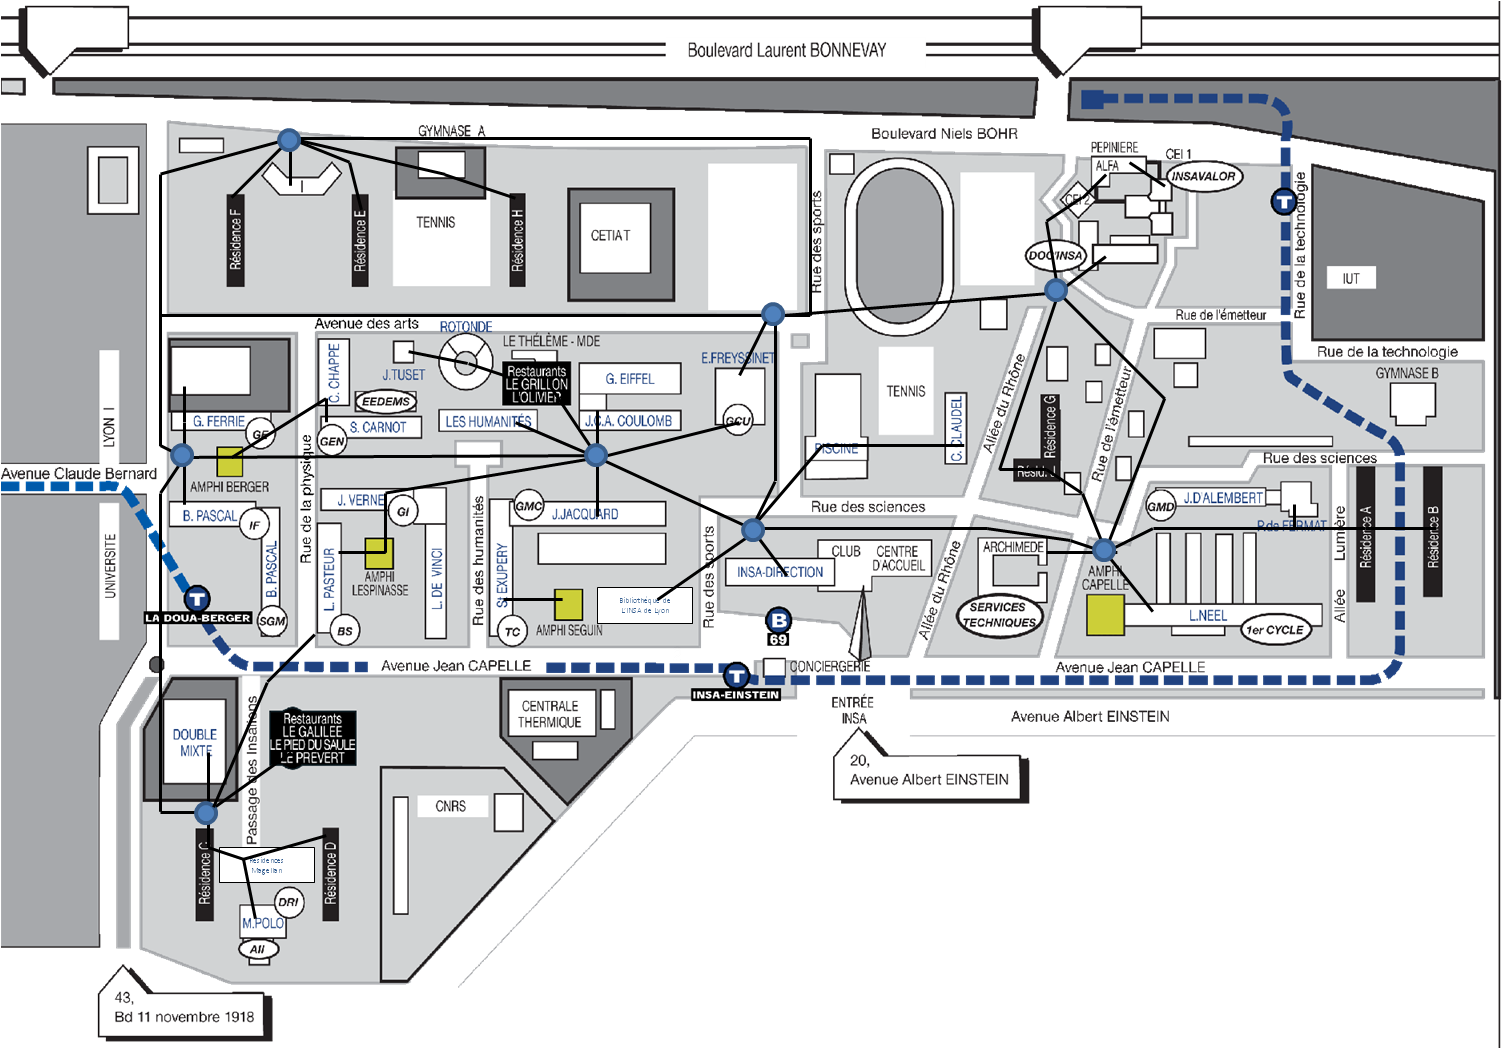
\includegraphics[scale=0.6]{Boucle1.png}
\end{figure}

\begin{figure}[h]
  \caption{\label{Plan_boucle2} Deuxième boucle optique}
  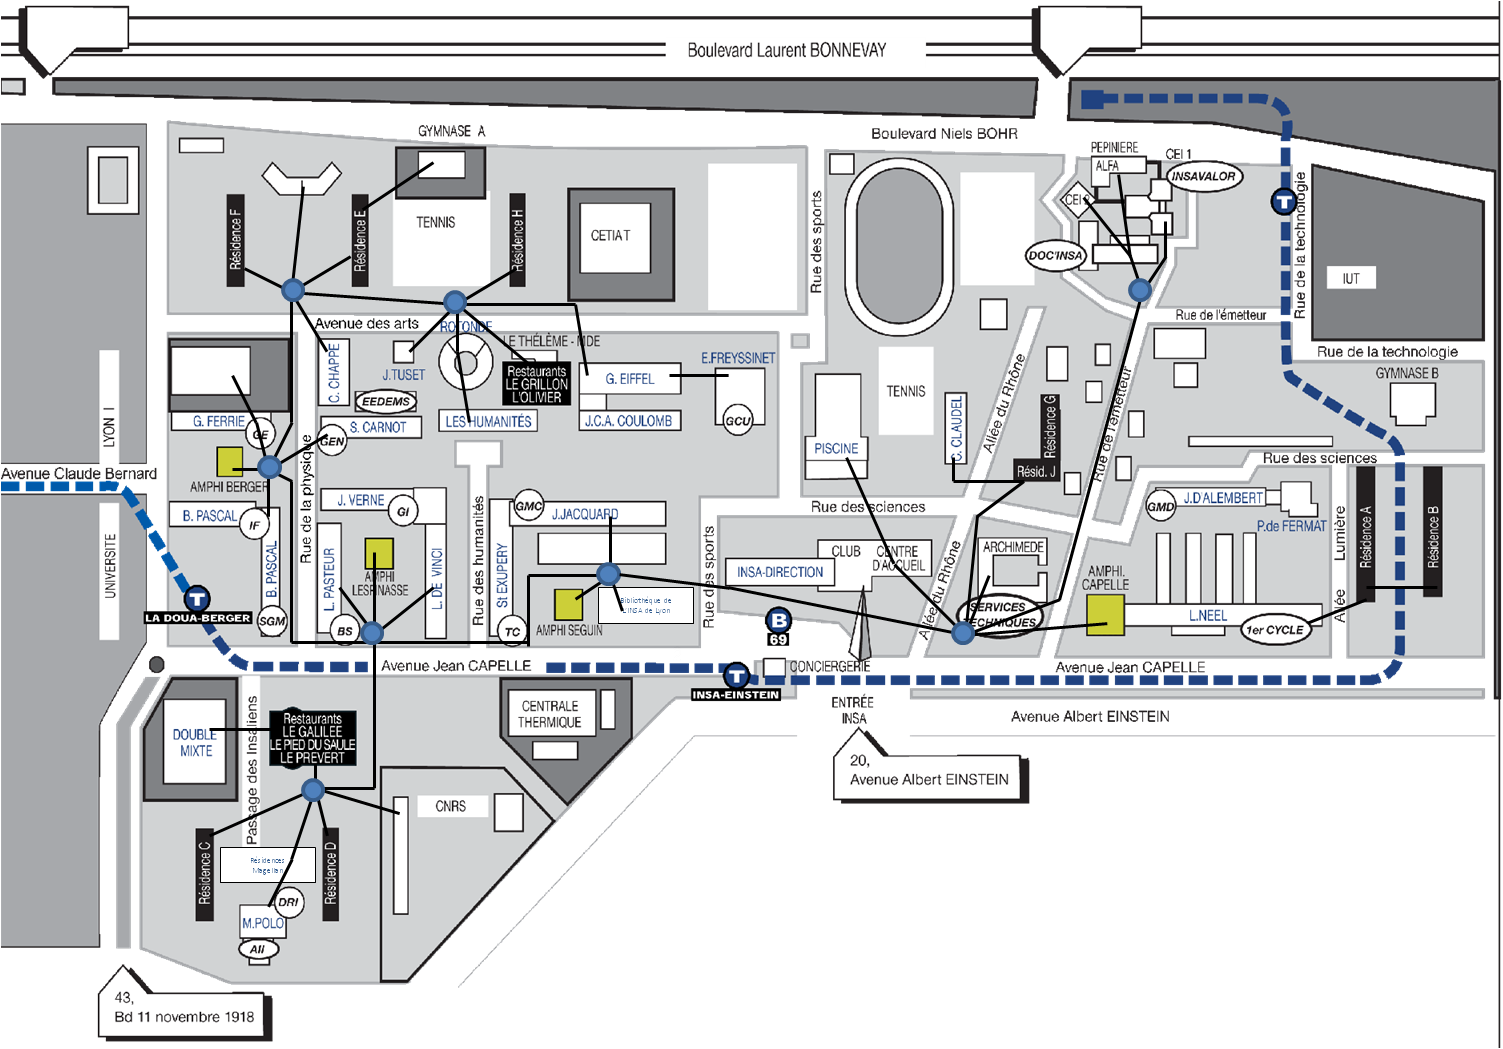
\includegraphics[scale=0.6]{Boucle2.png}
\end{figure}
\newpage

\paragraph{} Nous pouvons remarquer que le déploiement de ces boucles conduira à la construction de 15 noeuds optiques. Ces noeuds seront les points de convergence des fourreaux. Il seront composés de switchs optiques et de système de climatisation. L'alimentation électrique de ces noeuds se fera par cables électriques enterrés dans des fourreaux parallèles aux fourreaux de fibre optique. Cette connexion permettra non seulement de n'avoir à effectuer qu'une seule tranchée pour les fibres et l'alimentation mais également de permettre de centraliser l'alimentation des différents noeuds et locaux techniques au bâtiment Jacquard ce qui permettra d'y installer les équipements de protection en cas de coupure de courant sur le campus (onduleur sur batterie, groupe électrogène).
\paragraph{} Comme présenté dans les plans, les fourreaux seront placés entre les bâtiments connectés. Afin de limiter le nombre de noeuds optiques, certaines fibres passeront à l'intérieur d'un bâtiment et seront redirigées vers un autre fourreau de sortie dans le local technique de ce dernier pour connecter un bâtiment voisin. 
\paragraph{} La plupart des bâtiments du campus sont déjà équipés de locaux techniques pour la gestion de leur parc informatique. Lors de la mise en place des fourreaux pour la connexion d'un bâtiment, ces locaux tehniques seront rénovés et équipés avec le matériel nécessaire à la gestion des deux boucles. La rénovation passera par le changement des switchs qui seront utilisés par les téléphones en switchs POE, l'installation de climatisation dans les locaux (les switchs POE émettent plus de chaleur en fonctionnement que les switchs normaux).
\paragraph{} Si la place disponible dans les locaux techniques d'un bâtiment n'est pas suffisante, de nouveaux locaux pourront être créés après destruction des anciens. La politique sera alors la création d'un ou deux locaux techniques par bâtiment (en fonction de la taille de ce dernier). Ce locaux techniques seront situés le plus possible aux étages médians des bâtiments afin de limiter la longueur des câbles ethernet dans les bâtiments. 